\documentclass[aspectratio=169]{beamer}\usepackage[]{graphicx}\usepackage[]{xcolor}
% maxwidth is the original width if it is less than linewidth
% otherwise use linewidth (to make sure the graphics do not exceed the margin)
\makeatletter
\def\maxwidth{ %
  \ifdim\Gin@nat@width>\linewidth
    \linewidth
  \else
    \Gin@nat@width
  \fi
}
\makeatother

\definecolor{fgcolor}{rgb}{0.345, 0.345, 0.345}
\newcommand{\hlnum}[1]{\textcolor[rgb]{0.686,0.059,0.569}{#1}}%
\newcommand{\hlsng}[1]{\textcolor[rgb]{0.192,0.494,0.8}{#1}}%
\newcommand{\hlcom}[1]{\textcolor[rgb]{0.678,0.584,0.686}{\textit{#1}}}%
\newcommand{\hlopt}[1]{\textcolor[rgb]{0,0,0}{#1}}%
\newcommand{\hldef}[1]{\textcolor[rgb]{0.345,0.345,0.345}{#1}}%
\newcommand{\hlkwa}[1]{\textcolor[rgb]{0.161,0.373,0.58}{\textbf{#1}}}%
\newcommand{\hlkwb}[1]{\textcolor[rgb]{0.69,0.353,0.396}{#1}}%
\newcommand{\hlkwc}[1]{\textcolor[rgb]{0.333,0.667,0.333}{#1}}%
\newcommand{\hlkwd}[1]{\textcolor[rgb]{0.737,0.353,0.396}{\textbf{#1}}}%
\let\hlipl\hlkwb

\usepackage{framed}
\makeatletter
\newenvironment{kframe}{%
 \def\at@end@of@kframe{}%
 \ifinner\ifhmode%
  \def\at@end@of@kframe{\end{minipage}}%
  \begin{minipage}{\columnwidth}%
 \fi\fi%
 \def\FrameCommand##1{\hskip\@totalleftmargin \hskip-\fboxsep
 \colorbox{shadecolor}{##1}\hskip-\fboxsep
     % There is no \\@totalrightmargin, so:
     \hskip-\linewidth \hskip-\@totalleftmargin \hskip\columnwidth}%
 \MakeFramed {\advance\hsize-\width
   \@totalleftmargin\z@ \linewidth\hsize
   \@setminipage}}%
 {\par\unskip\endMakeFramed%
 \at@end@of@kframe}
\makeatother

\definecolor{shadecolor}{rgb}{.97, .97, .97}
\definecolor{messagecolor}{rgb}{0, 0, 0}
\definecolor{warningcolor}{rgb}{1, 0, 1}
\definecolor{errorcolor}{rgb}{1, 0, 0}
\newenvironment{knitrout}{}{} % an empty environment to be redefined in TeX

\usepackage{alltt}
\usetheme{gotham}

	\usepackage{standalone}
	\usepackage{tikz}
	\usepackage{pgfplots}
	\usepackage{tabularray} % Typeset tabulars and arrays (contains equivalent of longtable, booktabs and dcolumn at least)
		\UseTblrLibrary{booktabs} % to load extra commands from booktabs
	\usepackage{changepage}
	\usepackage{minted}
		\definecolor{codeback}{rgb}{0.90,0.91,0.92}
		\definecolor{codebackdark}{rgb}{0.10,0.11,0.12}

	\newcommand{\famName}[1]{\textsc{#1}}
	\newcommand{\themename}{\textbf{\textsc{Gotham}}}
\IfFileExists{upquote.sty}{\usepackage{upquote}}{}
\begin{document}

\section{Informing Policy via Dynamic Models: Cholera in Haiti}

\begin{frame}{Introduction}
  \setbeamercovered{transparent}
  One of the most scientifically interesting types of SSMs are \emph{mechanistic models}.
  
  \begin{itemize}
    \item Used when we have some understanding of how a dynamic system evolves over time. 
    \item Useful in modern science, and have some advantages over machine learning models \citep{baker18,hogg24}:
    \begin{itemize}
      \item Accounting for known (but unobserved) features can improve model performance. 
      \item More intepretable. 
      \item Facilitates predictions of interventions and other counter-factuals. 
    \end{itemize}
  \end{itemize}
  \pause
  In this chapter, I demonstrate these capabilities by fitting mechanistic models to the 2010-2019 cholera outbreak in Haiti. 
\end{frame}

\begin{frame}{Cholera in Haiti}
 \begin{tabular}{cl}  
         \begin{tabular}{c}
           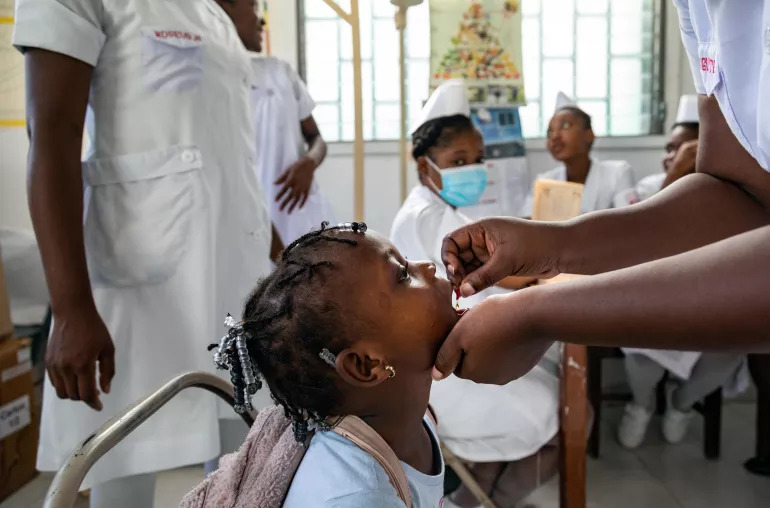
\includegraphics[height=4.3cm, width=5.5cm]{haiti/vaccination.jpeg}
           \end{tabular}
           & \begin{tabular}{l}
             \parbox{0.5\linewidth}{%  change the parbox width as appropiate
             \begin{itemize}
              \item Haiti experienced a cholera outbreak following the devastating 2010 earthquake. 
              \item From 2010-2019, more than \alert{800,000} recorded cases, making it one of the largest recorded outbreaks.
              \item Oral cholera vaccination (OCV) is available, but in limited supply.
              \item Image credit: \citet{unicef22}.
             \end{itemize}
    }
         \end{tabular}  \\
\end{tabular}
\end{frame}

\begin{frame}{Proposing interventions}
% At the time, there was interest in whether or not vaccinations would be a viable approach to eradicate cholera from Haiti.

A group of top researchers built three mechanistic models to estimate the potential impacts of various vaccination strategies \citep{lee20}.

\begin{itemize}
  \item 
\end{itemize}

\end{frame}

\end{document}
%EoF
